\section{Theory}

\subsection{Neural Networks}
The modern Neural Networks (NNs) are based on a mathematical model of the neuron, a socalled artificial neuron or perceptron.
This neuron receives multiple inputs \(\textbf{x}\) and applies a learnable weight \(w_{i}\) to each input, sums them up and adds a bias \(b\) to produce an output \(y\).
This information is then passed through a non-linear activation function \(f\) to introduce non-linearity into the model, allowing it to learn complex patterns in the data.
\begin{equation}
    y = f\left(\sum_{i=1}^{n} w_{i} x_{i} + b\right) = f ( \textbf{x} \cdot \textbf{w} + b )
\end{equation}
A common activation function is the Rectified Linear Unit (ReLU), defined as \(f(x) = \max(0, x)\).
In order to advance in high-dimensional problems, multiple layers of neurons are stacked together to form a deep neural network.
The arangement of these layers, called architecture, can vary widely and changes the way the network learns and processes information.
Usual architectures include feedforward networks, convolutional neural networks (CNNs) and recurrent neural networks (RNNs).
\begin{figure}
    \centering
    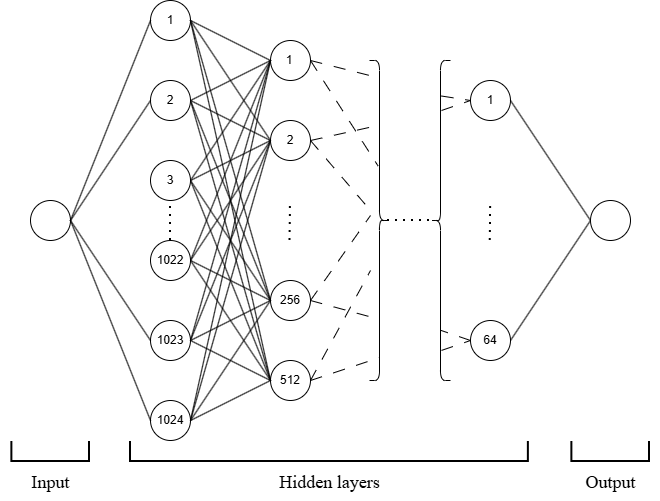
\includegraphics[width=0.8\textwidth]{images/NN.png}
    \caption{Schematic representation of a simple feedforward neural network with several hidden layers.}
\end{figure}

A better way to represent the architecture of a neural network is through matrix operations.
A hidden layer \(l\) with \(m\) neurons receives an input vector \(\textbf{a}^{(l-1)}\) of size \(n\) from the previous layer, applies a weight matrix \(\textbf{W}^{(l)}\) of size \(m \times n\) and a bias vector \(\textbf{b}^{(l)}\) of size \(m\), and produces an output vector \(\textbf{a}^{(l)}\) of size \(m\).
\begin{equation}
    \textbf{a}^{(l)} = f\left(\textbf{W}^{(l)} \cdot \textbf{a}^{(l-1)} + \textbf{b}^{(l)}\right)
\end{equation}

Stacking multiple layers allows the network to become a highly complex and non-linear function.
The combination of the non-linear activation functions and the learnable parameters (weights and biases) enables the network to approximate a wide variety of functions, making it a powerful tool for tasks such as classification, regression, and generative modeling.

\subsection{Training a Neural Network}
In order to improve the performance of a NN, it needs to be trained on a dataset. This process is realized by determining the optimal network parameters (weights \(\textbf{W}\) and biases \(\textbf{b}\)) that minimize a loss function \(\mathcal{L}\), which quantifies the difference between the predicted output and the true output.
A simple example of a loss function is the mean squared error (MSE) for regression tasks:
\begin{equation}
    \mathcal{L}_{MSE}(\hat{y}, y) = \frac{1}{N} \sum_{i=1}^{N} (\hat{y}_{i} - y_{i})^2
\end{equation}
where \(\hat{y}\) is the predicted output, \(y\) is the true output, and \(N\) is the number of samples in the dataset.

\begin{figure}
    \centering
    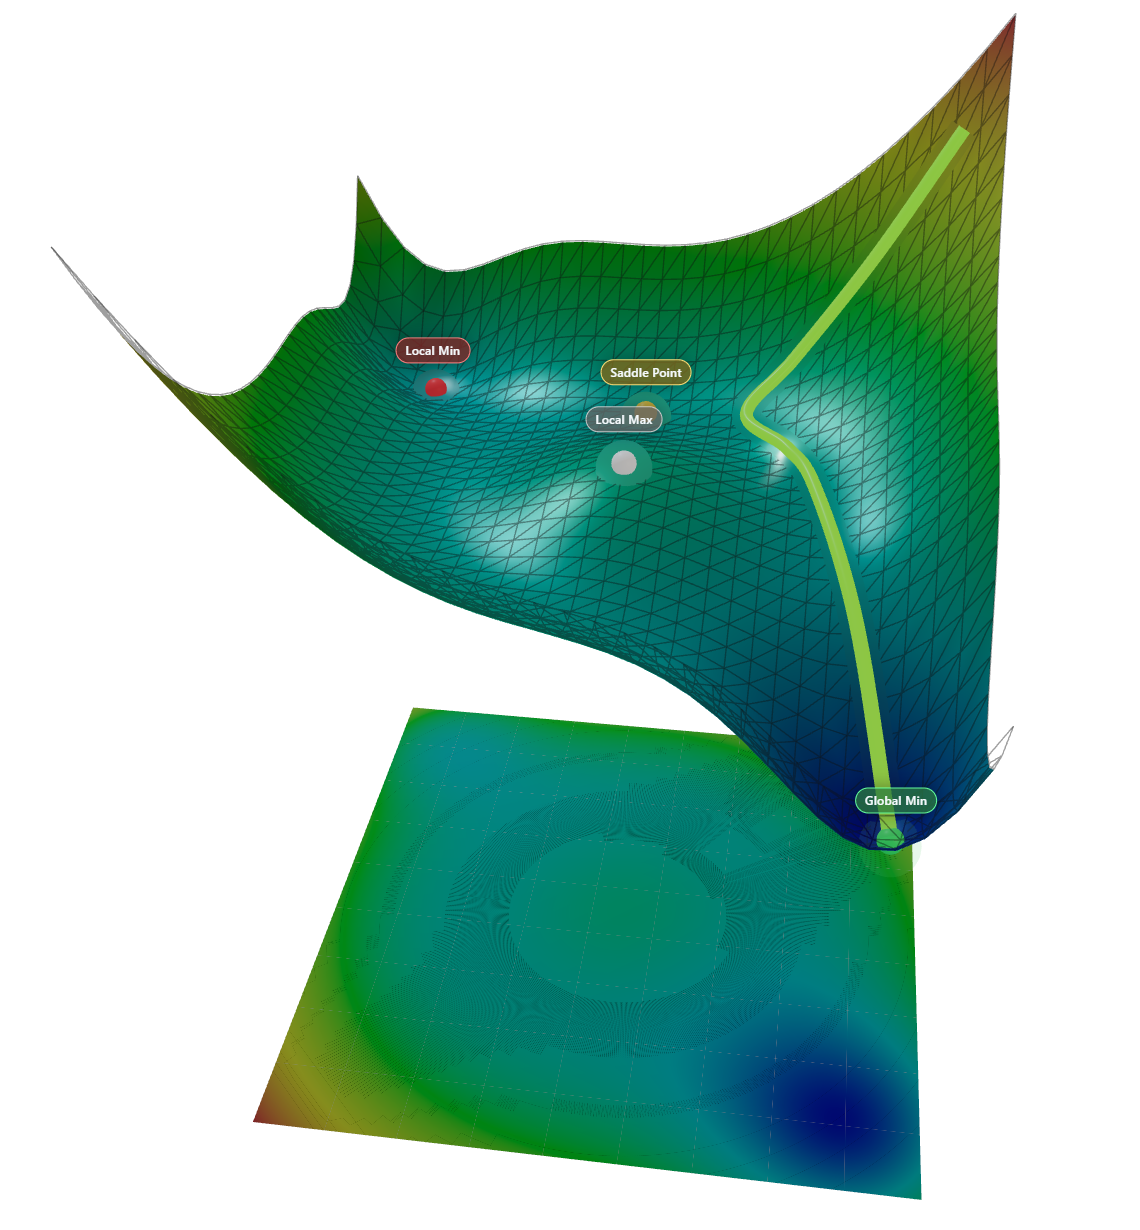
\includegraphics[width=0.8\textwidth]{images/PES.png}
    \caption{Schematic representation of the training process of a neural network, where the loss function is minimized by adjusting the weights and biases.}
\end{figure}

\subsection{Physics-Informed Neural Networks}

